%%%%%%%%%%%%%%%%%%%%%%%%%%%%%%%%%%%%%%%%%%%%%%%%%%%%%%%%%%%%%%%%
\section{System and Connections}
\label{sec:impl_system}

The \texttt{System} class assembles individual components into a running co-simulation scenario.
It implements the system abstraction introduced in Section~\ref{sec:architecture_system_connections} and realizes SR-03-01 and SR-03-02 (UR-03).
The event-connection functionality additionally supports the event-related interaction required by SR-04-02 (UR-04).

Figure~\ref{fig:impl_system_class} gives a class-level overview of the implementation objects involved in system composition and execution.
The structural analysis that derives the execution order from the registered connections is deferred to Section~\ref{sec:impl_structural}, and the master algorithms that consume this order are described in Section~\ref{sec:impl_algorithms}.

\begin{figure}[t]
    \centering
    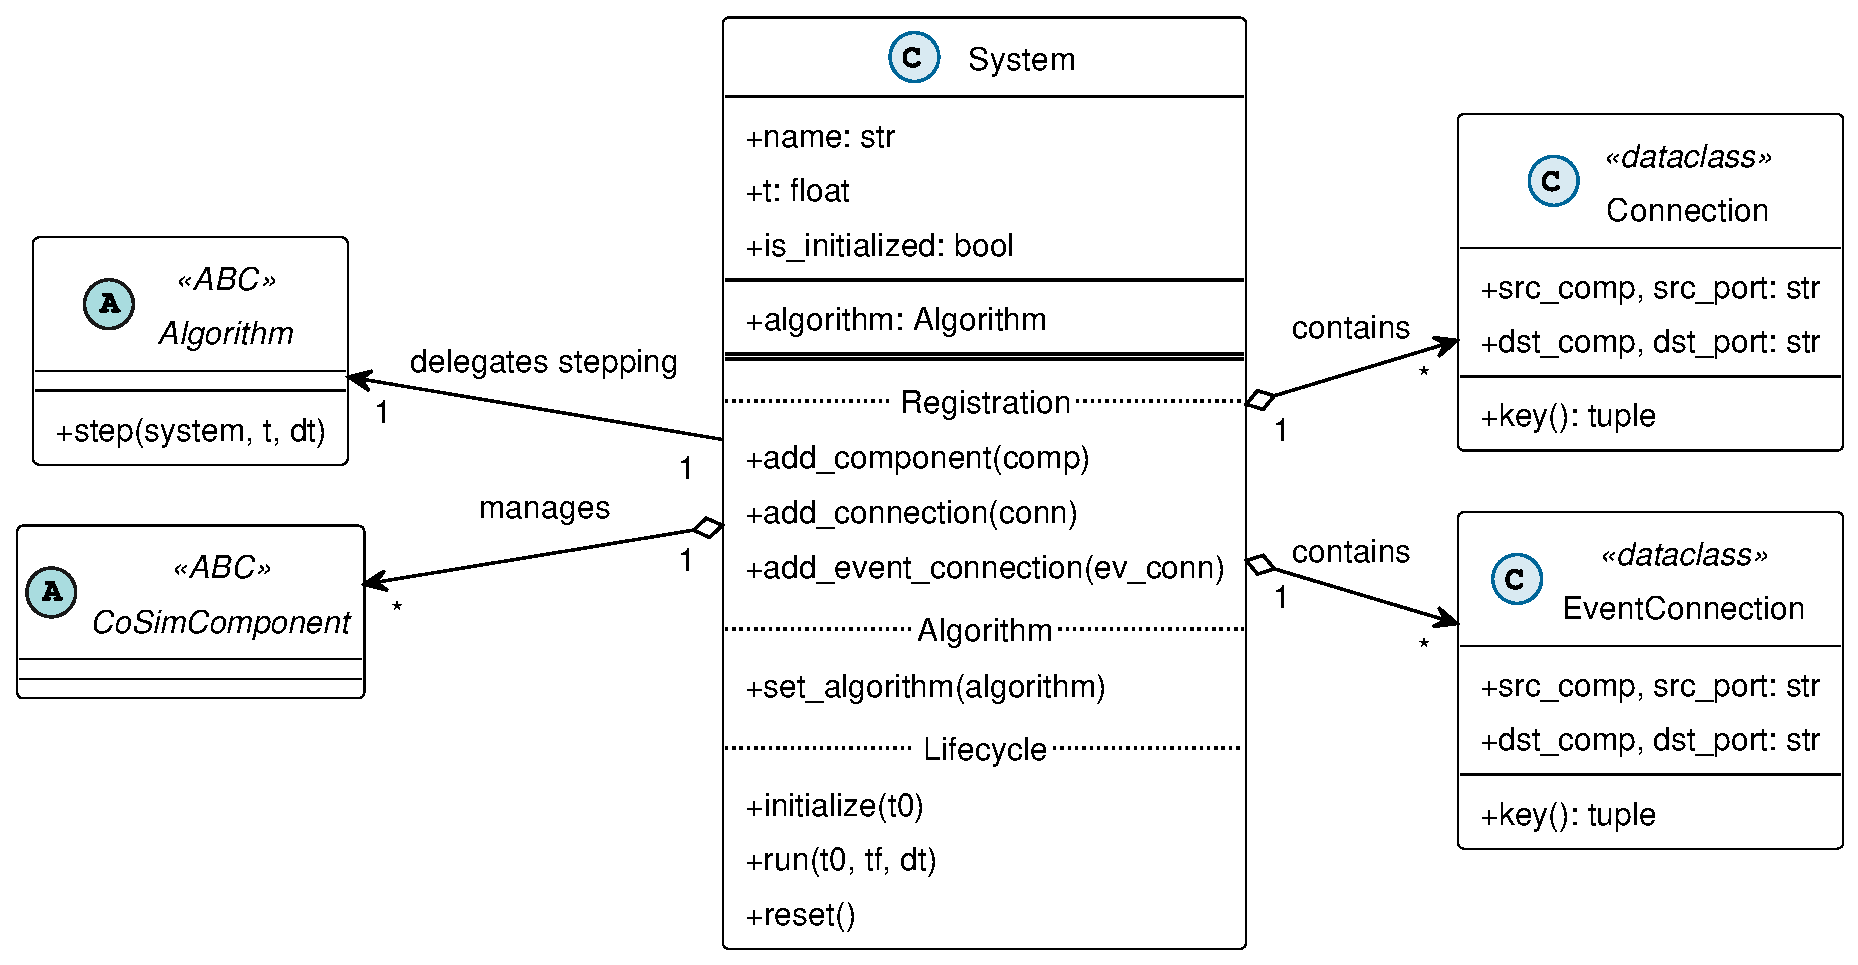
\includegraphics[width=0.85\textwidth]{diagrams/out/pdf/class/system/System.pdf}
    \caption{Class-level overview of the \texttt{System} abstraction in \syssimx. The diagram shows how the \texttt{System} manages components, stores signal and event connections, and delegates stepping to an \texttt{Algorithm}.}
    \label{fig:impl_system_class}
\end{figure}

%%%%%%%%%%%%%%%%%%%%%%%%%%%%%%%%%%%%%%%%%%%%%%%%%%%%%%
\subsection{Responsibilities and Stored State}

A \texttt{System} instance stores the structural definition of a co-simulation scenario.
This includes the registered components, signal connections, event connections, selected algorithm, and aggregated history.
It also tracks the current simulation time and the initialization state.
Derived metadata such as dependency graphs, algebraic loops, and execution order is introduced in Section~\ref{sec:impl_structural}.

%%%%%%%%%%%%%%%%%%%%%%%%%%%%%%%%%%%%%%%%%%%%%%%%%%%%%%
\subsection{Component Registration}

Components are registered with \texttt{add\_component()} before any connection can reference them.
Registration enforces that each component name is unique within the system and rejects additions after \texttt{initialize()} has been called, which keeps the structural analysis valid for the entire simulation run.
The component's history is registered with the system-level \texttt{SystemHistory} instance so that results from all components can be retrieved through a single call to \texttt{get\_history()} after the simulation.

%%%%%%%%%%%%%%%%%%%%%%%%%%%%%%%%%%%%%%%%%%%%%%%%%%%%%%
\subsection{Signal Connections}

A signal connection is represented by a immutable \texttt{Connection} object.
It stores the source component and output port together with the destination component and input port.
The object is frozen and hashable, so it can be used directly during duplicate checks and graph construction.

\paragraph{Validation.}
Signal connections are registered through \texttt{add\_connection()}.
Before a connection is stored, \texttt{\_validate\_connection()} checks that both components exist, both ports exist, the port specifications are compatible, and no duplicate connection is already registered.
The same validation also enforces single assignment.
A new connection is rejected if another connection already drives the same destination input.

\paragraph{Single Assignment.}
Each input port may be driven by at most one signal connection.
This invariant is enforced during connection registration.
The method \texttt{add\_connection()} rejects a new connection if another registered connection already targets the same destination component and input port.
This guarantees a unique source for every consumed input port.

%%%%%%%%%%%%%%%%%%%%%%%%%%%%%%%%%%%%%%%%%%%%%%%%%%%%%%
\subsection{Event Connections}

Hybrid scenarios use \texttt{EventConnection} to register a directed link from an event indicator of a source component to an event-handling target component.
The source port identifies the registered event indicator, and the destination port identifies the event input of the target that appears in the system graph.
The zero-crossing direction is not part of the connection.
It is defined once by the source component's event indicator and inherited by the generated event subscription.

The method \texttt{add\_event\_connection()} validates the connection, auto-subscribes the target, and updates the internal routing table from event source to target components.
The subscription is realized by appending a matching \texttt{Event} object to the target's \texttt{event\_subscriptions} list, which is the structure consumed by the hybrid algorithm of Section~\ref{sec:impl_hybrid}.
If a matching subscription is already present, it is not duplicated, so the same subscription can be expressed through manual registration or through \texttt{add\_event\_connection()} without conflicting entries on the target.
A duplicate event connection itself, however, is rejected at registration time.

%%%%%%%%%%%%%%%%%%%%%%%%%%%%%%%%%%%%%%%%%%%%%%%%%%%%%%
\subsection{Algorithm Selection}

The stepping algorithm is stored in the \texttt{algorithm} attribute and can be replaced through \texttt{set\_algorithm()}.
A \texttt{GaussSeidelAlgorithm} is installed at construction as a default that is appropriate for systems without state events.
At the start of \texttt{initialize()}, the system classifies the registered components into event sources, event listeners, and continuous-only components.
If any event sources are present, the algorithm is replaced by \texttt{HybridAlgorithm} irrespective of whether the user has set a different algorithm explicitly.
This ensures that the hybrid features of the framework are active whenever a component can produce state events and removes the need for the user to select the algorithm manually.

%%%%%%%%%%%%%%%%%%%%%%%%%%%%%%%%%%%%%%%%%%%%%%%%%%%%%%
\subsection{Lifecycle Orchestration}

Once all components and connections are registered, the system is driven through three phases.

\paragraph{Initialization.}
\texttt{initialize(t0)} first classifies the registered components and selects the hybrid algorithm when event sources are present.
It then prepares the component ports, computes direct-feedthrough metadata, and invokes the structural analysis of Section~\ref{sec:impl_structural}.
The resulting execution order is used to initialize the system generation by generation, as shown in Figure~\ref{fig:impl_system_initialization}.
For each generation, the system propagates upstream outputs, initializes the contained components, resolves local algebraic loops when needed, and performs a zero-step to publish outputs for downstream generations.
After initialization, the structural definition is fixed for the simulation run.

\begin{figure}[t]
  \centering
  \includegraphics[width=\linewidth]{diagrams/out/pdf/execution/System_Initialization.pdf}
  \caption[System initialization sequence.]{Sequence of operations executed by \texttt{System.initialize(t0)}.
    After classification, port preparation, and structural analysis, the system iterates over the execution order and, for each generation, propagates upstream outputs, initializes the contained components, resolves any algebraic loops, and performs a zero-step.
    The zero-step publishes direct-feedthrough outputs so that later generations are initialized with consistent input values.}
  \label{fig:impl_system_initialization}
\end{figure}

\paragraph{Run.}
\texttt{run(t0, tf, dt)} drives the coupled simulation by repeatedly delegating to the algorithm's \texttt{step()} method.
The stepping loop advances the time pointer in fixed macro steps of size \texttt{dt} and clamps the final step to the end time.
All orchestration details that depend on the chosen algorithm, such as input propagation between components, algebraic-loop iteration, and event localization, are owned by the algorithm (Section~\ref{sec:impl_algorithms}) and not by the \texttt{System} itself.

\paragraph{Reset.}
\texttt{reset()} releases the runtime state of the system without removing its structural definition.
It clears the aggregated history, resets all registered components through their own \texttt{reset()} hooks, and marks the system as not initialized.
The registered components, signal connections, event connections, and selected algorithm are retained, so the same scenario can be initialized and executed again without rebuilding the system configuration.

%%%%%%%%%%%%%%%%%%%%%%%%%%%%%%%%%%%%%%%%%%%%%%%%%%%%%%
\subsection{Verification}

The verification focuses on the registration contract of the \texttt{System}.
A valid registration must either extend the structural definition or be rejected before simulation state is changed.
The scenario uses lightweight mock components and checks signal connections, event connections, and lifecycle protection.
Table~\ref{tab:system_verification} summarizes the observed behavior.


\begin{table}[t]
  \centering
  \small
  \caption{Verification of the \texttt{System} registration contract.}
  \label{tab:system_verification}
  \begin{tabular}{p{3.2cm} p{6cm} p{6cm}}
    \toprule
    \textbf{Verified aspect} & \textbf{Minimal setup} & \textbf{Observed result} \\
    \midrule
    Signal connection registration
      & Three simple feedthrough components are registered.
        A valid connection from \texttt{A.y} to \texttt{C.u} is added.
        A second connection from \texttt{B.y} to the same input \texttt{C.u} is attempted.
      & The first connection is stored.
        The second connection is rejected with a \texttt{ValueError}.
        This confirms that each input port has a unique driver. \\
    \addlinespace

    Event connection registration
      & A hybrid source declares an event indicator.
        A hybrid listener declares a matching event input.
        An \texttt{EventConnection} links the source indicator to the listener input.
      & The target component receives exactly one matching event subscription.
        The subscription direction is inherited from the source event indicator.
        The connection itself only represents event routing. \\
    \addlinespace

    Lifecycle protection
      & The system is initialized after component and connection registration.
        A further component registration is attempted after initialization.
      & Initialization stores the system time and marks the system as initialized.
        Further component registration is rejected.
        The structural definition is therefore fixed for the simulation run. \\
    \bottomrule
  \end{tabular}
\end{table}

The scenario confirms that the registration contract is enforced uniformly across its three entry points.
The system rejects ambiguous or late structural changes before simulation starts, and event routing is configured through \texttt{EventConnection} while the event semantics remain owned by the source-side event indicator.
Structural-analysis properties are verified separately in Section~\ref{sec:impl_structural}.